\section{Ejemplos de los resultados}
A continuación, se muestra un ejemplo de cada uno de los resultadosobtenidos de la simulación del módulo \code{behavioral\_parkingController} para cada prueba del conjunto de pruebas mínimas detallado anteriormente. 
Para cada una de las pruebas descritas a continuación, se denota el tiempo de inicio y fin de la prueba dentro de la simulación de \code{gtkwave} con el formato (\code{tiempo de inicio de la prueba en segundos} : \code{tiempo de finalización de la prueba en segundos}).
Además, se utlizó el archivo \code{wave\_names.ttf} (Translate Filter File) para mostrar el nombre de cada señal en las formas de onda, lo cual facilita la lectura de las mismas.

\subsection{Funcionamiento normal básico (0:180)}
Se obtuvo la siguiente forma de onda:

\begin{figure}[!h]
    \centering
    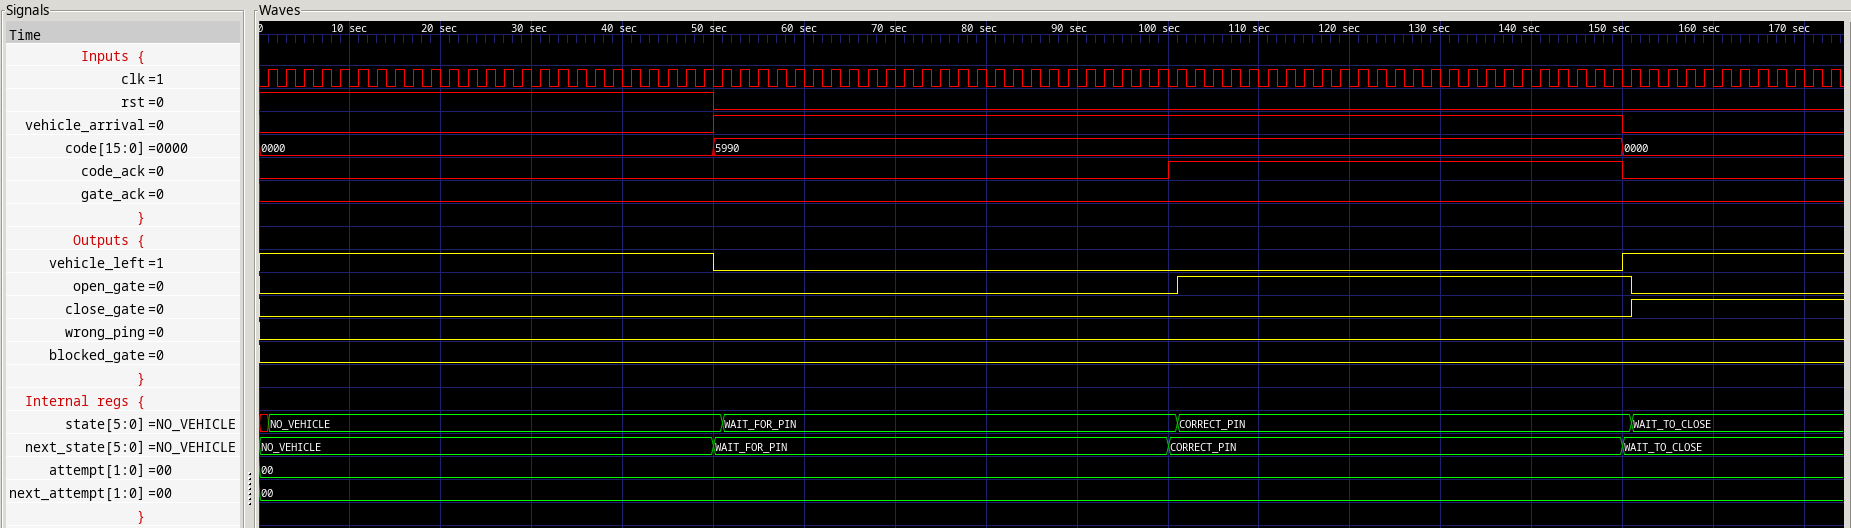
\includegraphics[width = \linewidth]{figs/prueba1.png}
    \caption{Forma de onda correspondiente a la prueba \#1: funcionamiento normal básico.}
    \label{fig3}
\end{figure}

Note que se autoriza correctamente que el vehículo entre al estacionamiento cuando ingresa el pin correcto.  

\newpage

\subsection{Ingreso de pin incorrecto menos de 3 veces (180:450)}
Se obtuvo la siguiente forma de onda:

\begin{figure}[!h]
    \centering
    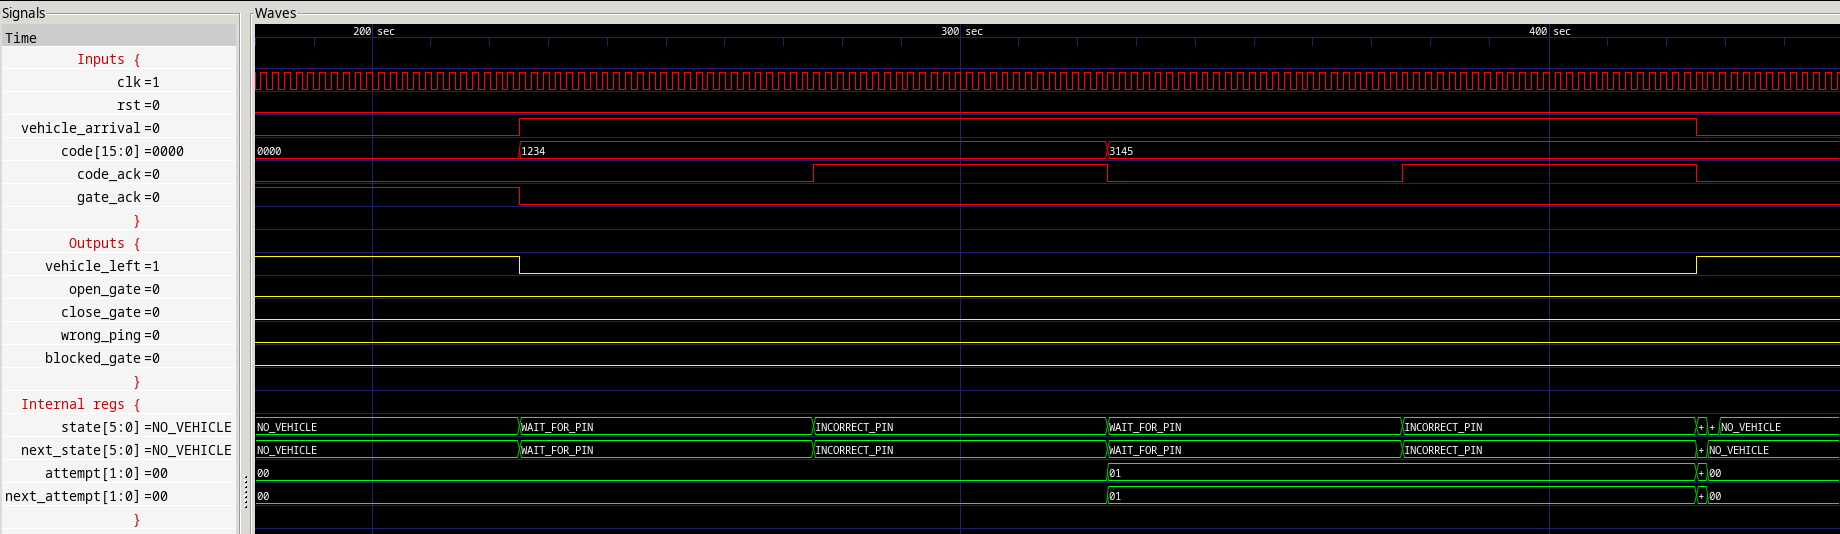
\includegraphics[width = \linewidth]{figs/prueba2.png}
    \caption{Forma de onda correspondiente a la prueba \#2: ingreso de pin incorrecto menos de 3 veces}
    \label{fig4}
\end{figure}

Note que no se autoriza que entre el vehículo al estacionamiento, y se incrementa \code{attempt} por cada intento fallido. 
Además, el controlador vuelve al estado \code{NO\_VEHICLE} cuando el vehículo se retira después de los dos intentos fallidos.
\subsection{Ingreso de pin incorrecto 3 o más veces (450:950)}
Se obtuvo la siguiente forma de onda:

\begin{figure}[!h]
    \centering
    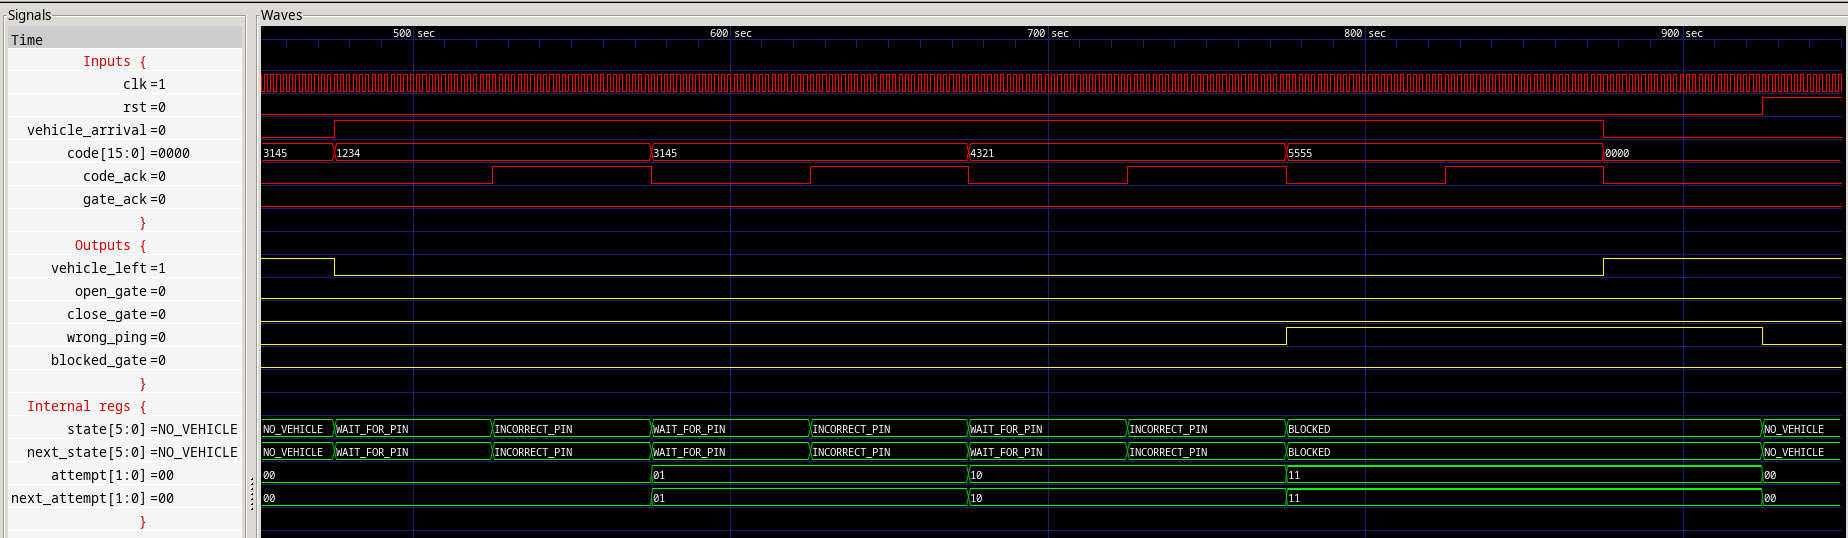
\includegraphics[width = \linewidth]{figs/prueba3.png}
    \caption{Forma de onda correspondiente a la prueba \#3: ingreso de pin incorrecto 3 o más veces.}
    \label{fig5}
\end{figure}

Note que el controlador llega al estado de bloqueo una vez que $\code{attempt} = 3$, y se activa la alarma \code{wrong\_ping}.
\subsection{Alarma de bloqueo (950:1225)}
Se obtuvo la siguiente forma de onda:

\begin{figure}[!h]
    \centering
    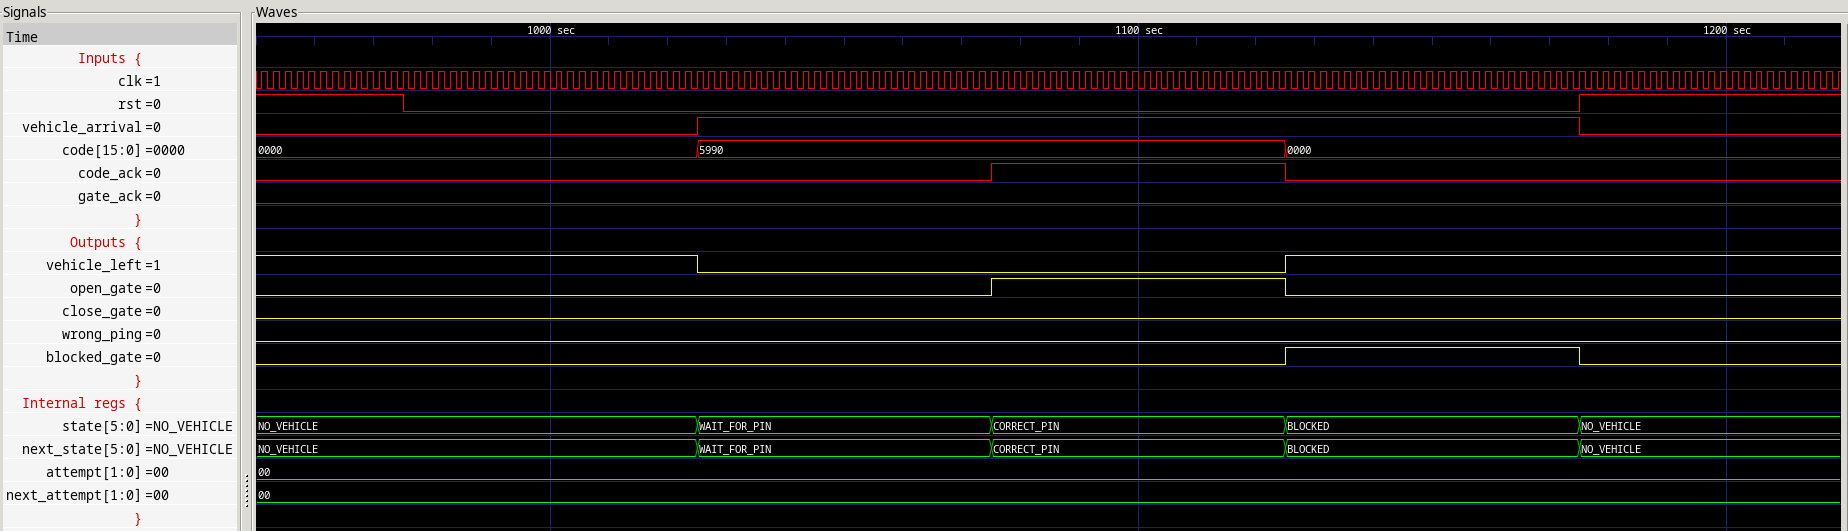
\includegraphics[width = \linewidth]{figs/prueba4.png}
    \caption{Forma de onda correspondiente a la prueba \#4: alarma de bloqueo.}
    \label{fig6}
\end{figure}

Note que el controlador llega al estado de bloqueo cuando \code{vehicle\_arrival} y \code{vehicle\_left} se ponen en alto a la misma vez, y se activa la alarma \code{blocked\_gate}.

